\documentclass{article}
\usepackage{amsmath,amssymb,subfig,mathrsfs,amsthm,graphicx}
\usepackage[draft]{hyperref}
\newcommand{\inner}[2]{\left\langle #1, #2 \right\rangle}
\newcommand{\tr}{\ensuremath\mathrm{tr}\,} 
\newcommand{\Span}{\ensuremath\mathrm{span}} 
\def\Re{\ensuremath{\mathrm{Re}}\,}
\def\Im{\ensuremath{\mathrm{Im}}\,}
\newcommand{\id}{\ensuremath\mathrm{id}} 
\newcommand{\diam}{\ensuremath\mathrm{diam}} 
\newcommand{\lcm}{\ensuremath\mathrm{lcm}} 
\newcommand{\supp}{\ensuremath\mathrm{supp}\,}
\newcommand{\dom}{\ensuremath\mathrm{dom}\,}
\newcommand{\upto}{\nearrow}
\newcommand{\downto}{\searrow}
\newcommand{\norm}[1]{\left\Vert #1 \right\Vert}
\newtheorem{theorem}{Theorem}
\newtheorem{lemma}[theorem]{Lemma}
\newtheorem{proposition}[theorem]{Proposition}
\newtheorem{corollary}[theorem]{Corollary}
\theoremstyle{definition}
\newtheorem{definition}[theorem]{Definition}
\newtheorem{example}[theorem]{Example}
\begin{document}
\title{The profinite completion of the integers, the $p$-adic integers, and Pr\"ufer $p$-groups}
\author{Jordan Bell}
\date{December 3, 2017}

\maketitle

\section{Topological rings and inverse systems}
By a \textbf{topological ring} we mean a ring $X$ with a Hausdorff topology such that $(x,y) \mapsto x+y, x \mapsto -x, (x,y) \mapsto x\cdot y$ 
are continuous. A \textbf{morphism} of topological rings is a continuous homomorphism of rings. 
An \textbf{inverse system} of topological rings is a family of topological rings
$X_i$ and a family of morphisms $\pi_{i,j}:X_i \to X_j$ for $i,j \in I$ with $i \geq j$, such that when $i \geq j \geq k$,
\[
\pi_{i,k} = \pi_{j,k} \circ \pi_{i,j}.
\]

If $Y$ is a topological ring,
we say that a family of morphisms $\psi_i:Y \to X_i$ is \textbf{compatible} with the inverse system if, whenever $i \geq j$,
\[
\pi_{i,j} \circ \psi_i = \psi_j.
\]

A topological ring $X$ and a compatible family of morphisms $\pi_i:X \to X_i$ is said to be an \textbf{inverse limit} of the inverse system
if whenever $Y$ is a topological ring and $\psi_i:Y \to X_i$ is a compatible family of morphisms, there is a unique 
morphism $\psi:Y \to X$ such that for all $i$,
\[
\pi_i \circ \psi = \psi_i.
\]
If $(X,\pi_i),(Y,\psi_i)$ are inverse limits of an inverse system, 
one checks that there is a unique isomorphism $\psi:X \to Y$ such that $\psi_i \circ \psi = \pi_i$ for all $i$.\footnote{Luis Ribes and Pavel Zalesskii, {\em Profinite Groups}, second ed., Chapter 1, ``Inverse and Direct Limits'', p.~2, Proposition 1.1.1 (b).}
If at least one inverse limit exists for an inverse system,
we
permit ourselves to speak about \textbf{the} inverse limit of the inverse system.

For showing that the inverse limit of an inverse system exists and for establishing properties of the inverse
limit, rather than stating that it is an object satisfying a universal property we can construct it in the following
way. Let $X$ be those $x \in \prod_{i \in I} X_i$ such that for $i \geq j$,
\[
\pi_{i,j}(x_i) = x_j.
\]
It is straightforward to check that $X$ is a subring of $\prod_{i \in I} X_i$ and that with the subspace topology inherited from the direct product
it is a topological ring.
We define $\pi_i:X \to X_i$ by $\pi_i = p_i \circ \iota$, where 
$\iota:X \to \prod_{i \in X_i}$ is the inclusion map and
$p_i: \prod_{j \in I} X_j \to X_i$ is the projection map. One checks that the morphisms $\pi_i$ are compatible with the inverse system, and then that 
$X$ together with this family of morphisms is an inverse limit of the inverse system.\footnote{Luis Ribes and Pavel Zalesskii, {\em Profinite Groups}, second ed., Chapter 1, ``Inverse and Direct Limits'', p.~2, Proposition 1.1.1 (a).}
This establishes that the inverse system has an inverse limit. Furthermore, 
one proves that $X$ is a closed subset of $\prod_{i \in I} X_i$.\footnote{Luis Ribes and Pavel Zalesskii, {\em Profinite Groups}, second ed., Chapter 1, ``Inverse and Direct Limits'', p.~3, Lemma 1.1.2.}
This lets us deduce properties of the inverse limit from  weakly hereditary properties of the direct product.



\section{Profinite rings}
A \textbf{profinite ring} is a topological ring that is the inverse limit of an inverse system of finite topological rings; since we demand that
topological rings be Hausdorff, being finite implies having the discrete topology. Suppose that
$X_i$ with morphisms $\pi_{i,j}$, $i \geq j, i,j \in i$, are an inverse system of finite topological rings.
Because $X_i$ is finite it is compact, so the direct product $\prod_{i \in I} X_i$ is compact. As the inverse limit $X$ of this inverse system is a closed
subset of the direct product, $X$ is a compact topological space.

A topological space is called \textbf{totally disconnected} if a subset being connected implies that the subset contains at most one point .In other
words, a topological space is totally disconnected if its connected components are all the singletons. 
One checks that a discrete topological space is totally disconnected, and that a product of totally disconnected spaces is totally
disconnected, and that being totally disconnected is hereditary.\footnote{Stephen Willard, {\em General Topology}, p.~210, \S 29.}
Therefore, a profinite ring is compact and totally disconnected.\footnote{In fact, a totally disconnected compact group
must be an inverse limit of finite discrete groups: Markus Stroppel, {\em Locally Compact Groups}, p.~172.}



\section{Profinite completion of the integers}
With the discrete topology, $\mathbb{Z}/n$ is a topological ring.
For $m|n$, we take $\phi_{n,m}:\mathbb{Z}/n \to \mathbb{Z}/m$ to be the projection map. 
The topological rings
$\mathbb{Z}/n$ and the morphisms $\phi_{n,m}$ are an inverse system in the category of topological rings (ordering the indices by  $n \geq m$ when $m|n$), and we denote the inverse
limit by $\widehat{\mathbb{Z}}$, with morphisms $\phi_n:\widehat{\mathbb{Z}} \to \mathbb{Z}/n$ satisfying
\[
\phi_{n,m} \circ \phi_n = \phi_m, \qquad m|n,
\]
called the \textbf{profinite completion of $\mathbb{Z}$}. 
$\widehat{\mathbb{Z}}$ is a profinite ring, hence it is compact and totally disconnected, and because the inverse system consists of countably many metrizable limitands,
the direct product $\prod_{n=1}^\infty \mathbb{Z}/n$ and thus the inverse limit is metrizable.

Let $\psi_n:\mathbb{Z} \to \mathbb{Z}/n$ be the projection map. For $m|n$, 
\[
\phi_{n,m} \circ \psi_n = \psi_m.
\]
Namely, the morphisms $\psi_n$ are compatible with the inverse system. 
For example,
\[
\phi_{15,3} \circ \psi_{15}(22) = \phi_{15,3}(7+(15)) = 1+(3) = \psi_3(22).
\]
Hence there is a unique morphism $\psi:\mathbb{Z} \to \widehat{\mathbb{Z}}$ such that for all $n \geq 1$,
\[
\phi_n \circ \psi = \psi_n.
\]
If $a,b \in \mathbb{Z}$ and $a \neq b$, there is some $n$ such that $a \not \equiv b \pmod{n}$, that is, $\psi_n(a) \neq \psi_n(b)$. 
It must then be that $\psi(a) \neq \psi(b)$. Therefore, $\psi$ is one-to-one.

Because $\widehat{\mathbb{Z}}$ is compact and metrizable it is separable. 
We prove that the image of $\mathbb{Z}$ in its profinite completion is dense, which explicitly displays a  countable dense subset.\footnote{Brian Osserman,
{\em Inverse limits and profinite groups},
\url{https://www.math.ucdavis.edu/~osserman/classes/250C/notes/profinite.pdf}}

\begin{theorem}
$\psi(\mathbb{Z})$ is a dense subset of $\widehat{\mathbb{Z}}$.
\end{theorem}
\begin{proof}
Let $U$ be a nonempty subset of $\widehat{\mathbb{Z}}$. $\widehat{\mathbb{Z}}$ has the subspace topology inherited
from the direct product $\prod_{n=1}^\infty \mathbb{Z}/n$,
so 
there are open sets $V_n$ in $\mathbb{Z}/n$, where there are only finitely many $n$ such that $V_n \neq \mathbb{Z}/n$,
such that for $V = \prod_{n=1}^\infty V_n$, the set $\widehat{\mathbb{Z}} \cap V$ is nonempty and is contained in $U$. 
To prove that $\psi(\mathbb{Z})$ is dense in $\widehat{\mathbb{Z}}$ it will suffice to prove that
there is some $a \in \mathbb{Z}$ such that $\psi(a) \in \widehat{\mathbb{Z}} \cap V \subset  U$. 

Take $n_0$ such that for $n > n_0$, $V_n = \mathbb{Z}/n$. (In this proof by $\geq$ we mean the usual order on the positive integers, not $n \geq m$ when
$m|n$.)
Because  $\widehat{\mathbb{Z}} \cap V$ is nonempty, there is some $x \in  \widehat{\mathbb{Z}} \cap V$. 
Let $N=\lcm(1,2,\ldots,n_0)$ and let $a \in \psi_N^{-1}(\phi_N(x)) \subset \mathbb{Z}$. For $1 \leq n \leq n_0$,  $n|N$ and
\begin{align*}
\phi_n(\psi(a))&=(\phi_{N,n} \circ \phi_N)(\psi(a))\\
&=(\phi_{N,n} \circ \phi_N \circ \psi)(a)\\
&=(\phi_{N,n} \circ \psi_N)(a)\\
&=\phi_{N,n}(\psi_N(a))\\
&=\phi_{N,n}(\phi_N(x))\\
&=(\phi_{N,n} \circ \phi_N)(x)\\
&=\phi_n(x).
\end{align*}
Hence $\phi_n(\psi(a)) \in V_n$, and so $\psi(a) \in V$.
$\psi:\mathbb{Z} \to \widehat{\mathbb{Z}}$ so  $\psi(a) \in \widehat{\mathbb{Z}}$. Therefore,
$\psi(a) \in \widehat{\mathbb{Z}} \cap V$, which proves the claim.
\end{proof}




\section{{\em p}-adic integers}
Let $p$ be a prime. $\mathbb{Z}/p^n$ with the discrete topology is a topological ring. 
For $n \geq m$, let $\pi_{n,m}:\mathbb{Z}/p^n \to \mathbb{Z}/p^m$
be the projection map. For example, with $p=3$,
\[
\pi_{3,2}(15+(3^3)) = 6+(3^2).
\]
The topological rings $\mathbb{Z}/p^n$ and the morphisms $\pi_{n,m}$ are an inverse system in the category of topological rings. 
The inverse limit of this inverse system is a topological ring denoted by $\mathbb{Z}_p$, together with morphisms
$\pi_n:\mathbb{Z}_p \to \mathbb{Z}/p^n$ such that
\[
\pi_{n,m} \circ \pi_n = \pi_m
\]
 for $n \geq m$.
We call $\mathbb{Z}_p$ the \textbf{ring of $p$-adic integers}. It is compact and totally disconnected. 
Furthermore, because each limitand $\mathbb{Z}/p^n$ is metrizable by the discrete metric, the countable direct product
$\prod_{n=1}^\infty \mathbb{Z}/p^n$ is metrizable, and therefore so is $\mathbb{Z}_p$. 

Let $\chi_n:\mathbb{Z} \to \mathbb{Z}/p^n$ be the projection maps. For $n \geq m$,
\[
\pi_{n,m} \circ \chi_n = \chi_m.
\]
Namely,  the morphisms $\chi_n$ are compatible with the inverse system, and therefore there is a unique morphism 
$\chi:\mathbb{Z} \to \mathbb{Z}_p$ such that for all $n \geq 1$,
\[
\pi_n \circ \chi = \chi_n.
\]
If $a,b \in \mathbb{Z}$ and $a \neq b$, there is some $n$ such that $a \not \equiv b \pmod{p^n}$, so that
$\chi_n(a) \neq \chi_n(b)$, whence $\chi(a) \neq \chi(b)$. This shows that $\chi:\mathbb{Z} \to \mathbb{Z}_p$ is one-to-one.
Furthermore, like how the  image  of $\mathbb{Z}$ in $\widehat{\mathbb{Z}}$ is dense,
the image of $\mathbb{Z}$ in $\mathbb{Z}_p$ is dense.

\begin{theorem}
$\chi(\mathbb{Z})$ is a dense subset of $\mathbb{Z}_p$. 
\end{theorem}


\section{The Chinese remainder theorem}
For $n$ a positive integer, let $v_p(n)$ denote the highest power of the prime $p$ that divides $n$. For example, $v_3(45)=2$
and $v_3(11)=0$. The \textbf{Chinese remainder theorem} states that
\[
\mathbb{Z}/n \cong  \prod_p \mathbb{Z}/p^{v_p(n)}.
\]
Then, supposing that the following steps are correct,\footnote{See Paul Garrett, {\em The ur-solenoid and the adeles},
\url{http://www.math.umn.edu/~garrett/m/mfms/notes/04_ur_solenoid.pdf}}
\[
\widehat{\mathbb{Z}}  = \varprojlim_n \mathbb{Z}/n 
\cong \varprojlim_n \prod_p \mathbb{Z}/p^{v_p(n)}
\cong \prod_p \varprojlim_\nu \mathbb{Z}/p^{\nu}
\cong \prod_p \mathbb{Z}_p
\]
as topological rings.


\section{Direct systems}
A \textbf{direct system} of abelian groups  is a family of abelian groups
$A_i$ and a family of group homomorphisms $\phi_{i,j}:A_i \to A_j$ for $i,j \in I$ with $i \leq j$, such that when $i \leq j \leq k$,
\[
\phi_{i,k} = \phi_{j,k} \circ \phi_{i,j}.
\]

If $A$ is an abelian group,
we say that a family of group homomorphisms $\psi_i:A_i \to A$ is \textbf{compatible} with the direct system if, whenever $i \leq j$,
\[
 \psi_j \circ \phi_{i,j}  = \psi_i.
\]

An abelian group $A$ and a compatible family of group homomorphisms $\phi_i:A_i \to A$ is said to be a \textbf{direct limit} of the direct system
if whenever $B$ is an abelian group and $\psi_i:A_i \to B$ is a compatible family of group homomorphisms, there is a unique 
group homomorphism $\psi:A \to B$ such that for all $i$,
\[
\psi \circ \phi_i = \psi_i.
\]
It can be proved that a direct system of abelian groups has a direct limit, and that if
if $(A,\phi_i),(B,\psi_i)$ are direct limits of a direct system, 
then there is a unique group isomorphism $\psi:A \to B$ such that
$\psi_i  = \psi \circ \phi_i$ for all $i$.\footnote{Luis Ribes and Pavel Zalesskii, {\em Profinite Groups}, second ed., Chapter 1, ``Inverse and Direct Limits'', p.~15,
Proposition 1.2.1.}
We
permit ourselves to speak about \textbf{the} direct limit of the direct system.


\section{Pontryagin duality}
A \textbf{morphism} of a locally compact abelian group is a continuous group homomorphism.
Let $S^1=\{z \in \mathbb{C}: |z|=1\}$. The \textbf{Pontryagin dual} of a locally compact abelian group $G$
is the collection of morphisms $G \to S^1$, where we define
$\phi_1 \phi_2$ by $(\phi_1 \phi_2)(x)=\phi_1(x)\phi_2(x)$. 

It is a fact that
if $G_i$ is an inverse system of compact abelian groups with surjective morphisms $G_i \to G_j$ for $i \geq j$, then 
the Pontryagin dual of the inverse limit is isomorphic to the direct limit of the Pontryagin duals of the $G_i$, and that the
direct limit is equal to the union of the images of the Pontryagin duals.\footnote{Karl H. Hofmann and Sidney A. Morris,
{\em The Structure of Compact Groups}, 2nd revised and augmented edition, p.~24, Proposition 1.36.}

The Pontryagin dual of the compact abelian group $\mathbb{Z}/N$ is isomorphic to the discrete abelian group $\mathbb{Z}/N$. (The discrete
topology on a finite abelian group is compact.) The dual of the inverse system  of projections
$\pi_{n,m}:\mathbb{Z}/p^n \to \mathbb{Z}/p^m$, $n \geq m$, is the direct system of inclusion maps
 $i_{m,n}:\mathbb{Z}/p^m \to \mathbb{Z}/p^n$, $m \leq n$, and the 
 direct limit of this direct system is a discrete abelian group denoted by $\mathbb{Z}(p^\infty)$, called the \textbf{Pr\"ufer $p$-group}, with morphisms $i_n:\mathbb{Z}/p^n \to \mathbb{Z}(p^\infty)$ and which satisfies
  \[
 \mathbb{Z}(p^\infty) = \bigcup_{n \in \mathbb{Z}^+} i_n(\mathbb{Z}/p^n).
 \]
 
 
 \section{Solenoids}
 For $n \geq 0$, let $\pi_n:\mathbb{R} \to \mathbb{R}/p^n \mathbb{Z}$ be the projection map, and give $\mathbb{R}/p^n \mathbb{Z}$ the final
 topology induced by this map, with which
$\mathbb{R}/p^n \mathbb{Z}$ is  a compact abelian group. 
 For $n \geq m$, let
 \[
 \varphi_{n,m}:\mathbb{R}/p^n \mathbb{Z} \to \mathbb{R}/p^m \mathbb{Z}
 \]
 be the projection map. The following diagram commutes:
 
\begin{figure}[h]
\begin{center}
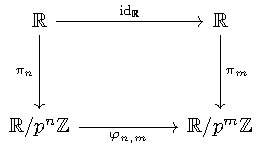
\includegraphics[width=0.4\textwidth]{tikz}
\end{center}
\end{figure}

It is immediate that the compact abelian groups $\mathbb{R}/p^n$ and the morphisms $\varphi_{n,m}$, $n \geq m$,
are an inverse system. We call the inverse limit of this sytem the \textbf{$p$-adic solenoid}, denoted
$\mathbb{T}_p$, with morphisms $\varphi_n:\mathbb{T}_p \to \mathbb{R}/p^n \mathbb{Z}$.\footnote{There are few books that present the $p$-adic solenoid. Two are Alain M. Robert, {\em A Course in $p$-adic Analysis}, p.~54, Appendix to Chapter 1, and
Karl A. Hofmann and Sidney A. Morris, {\em The Lie Theory of Connected Pro-Lie Groups}, p.~589, Example 14.4.}
$\mathbb{T}_p$ is a compact abelian group. 

One proves that each morphism $\varphi_n:\mathbb{T}_p \to \mathbb{R}/p^n \mathbb{Z}$ is onto. 
We now relate the $p$-adic solenoid to the $p$-adic integers.\footnote{Alain M. Robert, {\em A Course in $p$-adic Analysis}, p.~55, Appendix A.1.}
 $\mathbb{Z} \subset
 \mathbb{R}$ implies that $\mathbb{Z}/p^n = \mathbb{Z}/p^n \mathbb{Z} \subset
 \mathbb{R}/p^n\mathbb{Z}$. We model $\mathbb{Z}_p$ as a subset of the direct product
 $\prod \mathbb{Z}/p^n$ and model $\mathbb{T}_p$ as a subset of the direct product
 $\prod \mathbb{R}/p^n\mathbb{Z}$, and thus the statement of the following theorem makes sense.

\begin{theorem}
$\ker \varphi_n = p^n \mathbb{Z}_p$.
\end{theorem}



\end{document}